\subsection{Performance Analysis}
In order to give enough chance to communicate between \verb|node_1| and \verb|node_4|. I use \verb|setdest| tool to generate {\bf 70} nodes in the area \verb|350x350|.
\subsubsection{Delay Compare}
\begin{figure}[H]
    \centering
    \begin{tabular}{l r}
        \resizebox{60mm}{!}{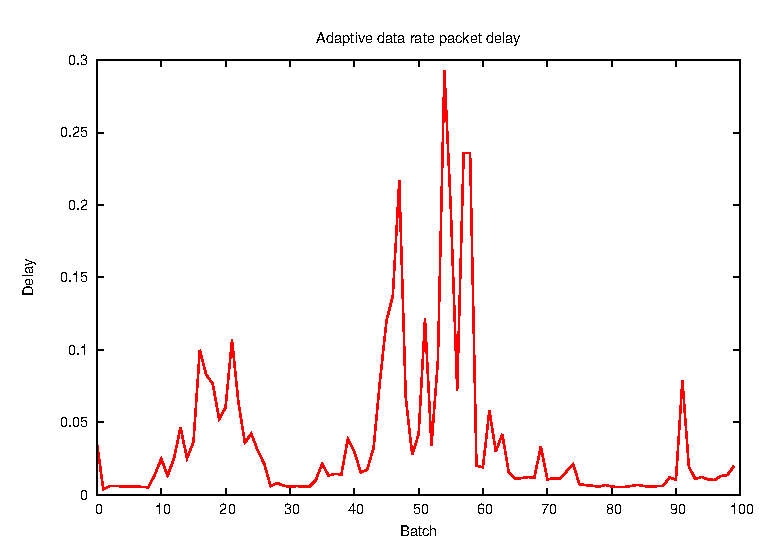
\includegraphics{eps/scenario_2/udp/ad_delay_bw.eps}} &
        \resizebox{60mm}{!}{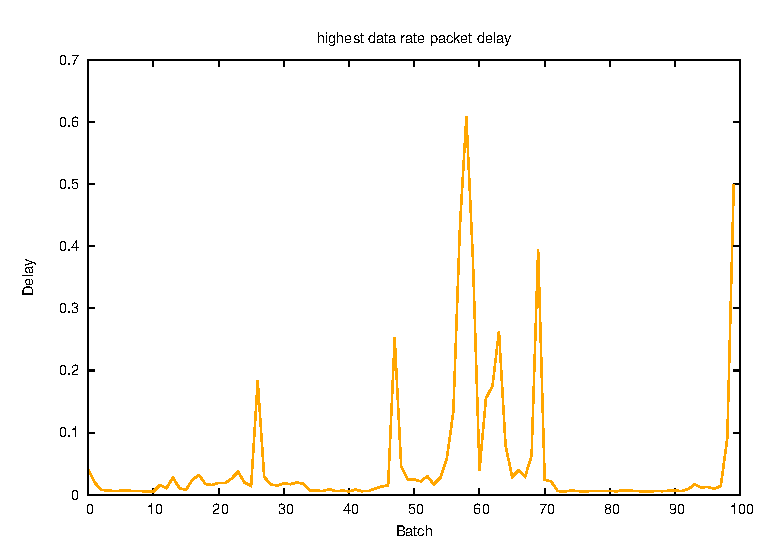
\includegraphics{eps/scenario_2/udp/hi_delay_bw.eps}} \\
        \multicolumn{2}{c}{\resizebox{60mm}{!}{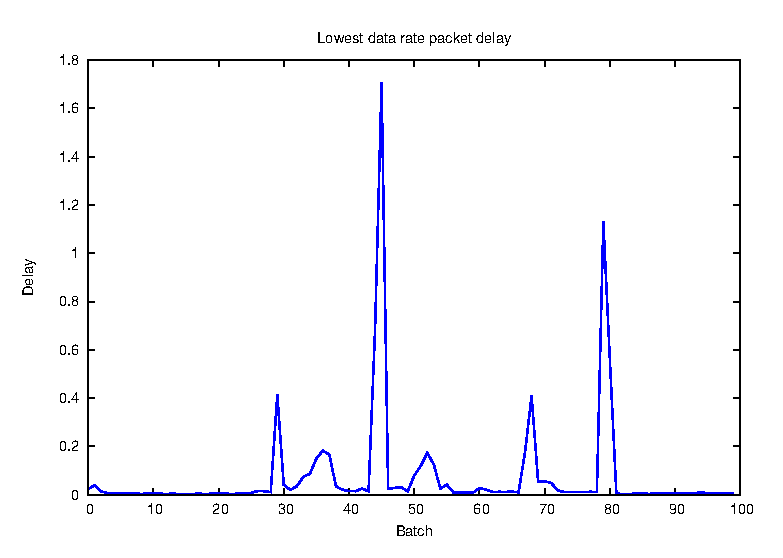
\includegraphics{eps/scenario_2/udp/lo_delay_bw.eps}}} 
    \end{tabular}
    \caption{Delay Compare}
\end{figure}

\begin{table}[H]
    \centering
    \setlength{\extrarowheight}{2mm}
    \addtolength{\tabcolsep}{3mm}
    \begin{tabular}{c c c}
        \hline \hline
        &  Avg & Stdev \\
        \hline
        AD & 0.056538 & 0.144655 \\
        HI & 0.062663 & 0.328750 \\
        LO & 0.155872 & 1.310392 \\
        \hline
    \end{tabular}
    \caption{Delay Compare}
\end{table}

Compare with static model. It is great changed. The average of delay of three case is smaller than previous static model. And the highest end-to-end delay when the delivery rate is lowest. The \verb|AD| case also between \verb|HI| and \verb|LO|. The delay vary sharply range [40,80]. To get the reason for this. I run the \verb|nam|. I found that \verb|node_1| and \verb|node_4| can communicate frequently during the period of time. After this stage, \verb|node_1| is far away from
\verb|node_4| so that they can not communicate. 

\subsubsection{Delay Jitter Compare}
\begin{figure}[H]
    \centering
    \begin{tabular}{l r}
        \resizebox{60mm}{!}{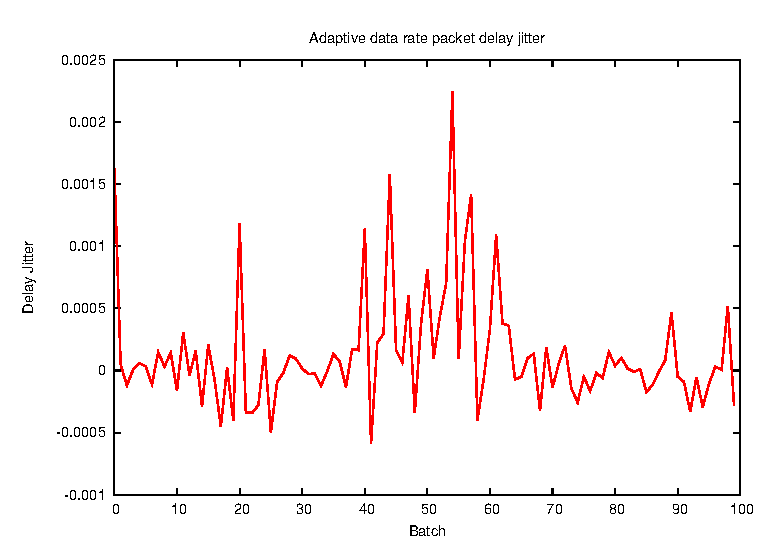
\includegraphics{eps/scenario_2/udp/ad_jitter_bw.eps}} &
        \resizebox{60mm}{!}{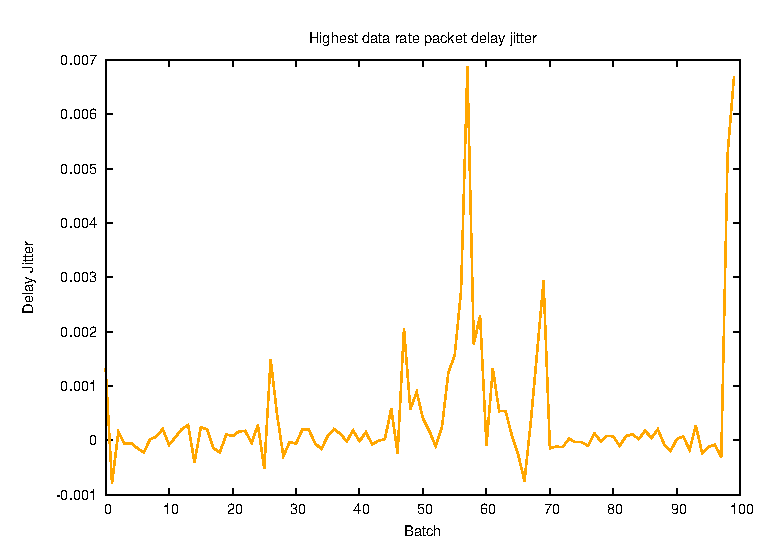
\includegraphics{eps/scenario_2/udp/hi_jitter_bw.eps}} \\
        \multicolumn{2}{c}{\resizebox{60mm}{!}{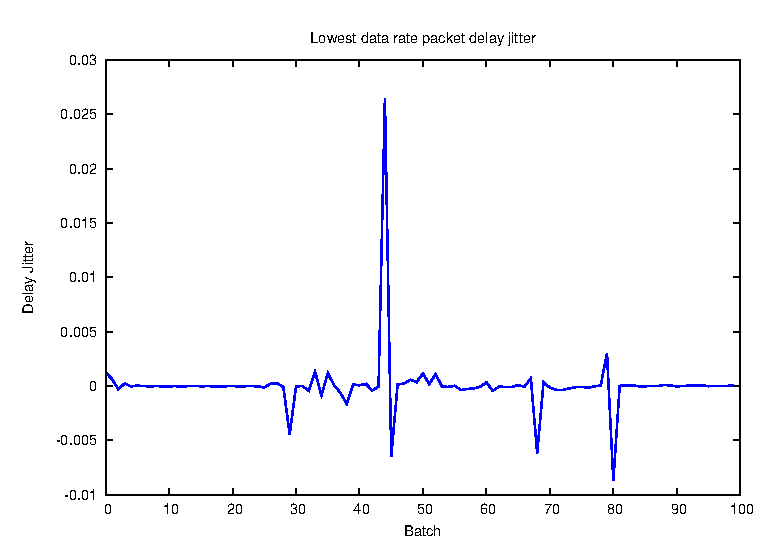
\includegraphics{eps/scenario_2/udp/lo_jitter_bw.eps}}} 
    \end{tabular}
    \caption{Delay jitter Compare}
\end{figure}

The jitter figure illustrate neatly that during approximately [40,80], \verb|node_1| and \verb|node_4| peak communicate probability occurs. During the initial stage, \verb|node_1| can not get touch with \verb|node_4|.

\subsubsection{Throughput Compare}
\begin{figure}[H]
    \centering
    \resizebox{90mm}{!}{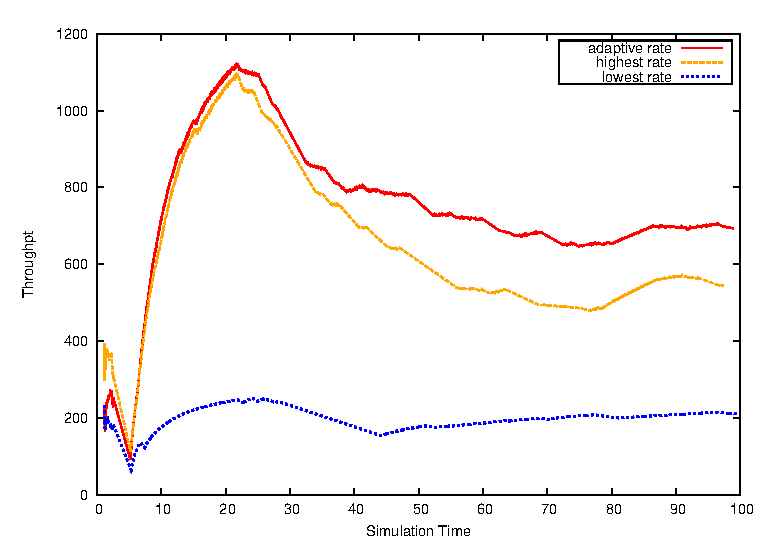
\includegraphics{eps/scenario_2/udp/throughput_bw.eps}}
    \caption{Throughput Compare}
\end{figure}

\begin{figure}[H]
    \centering
    \resizebox{90mm}{!}{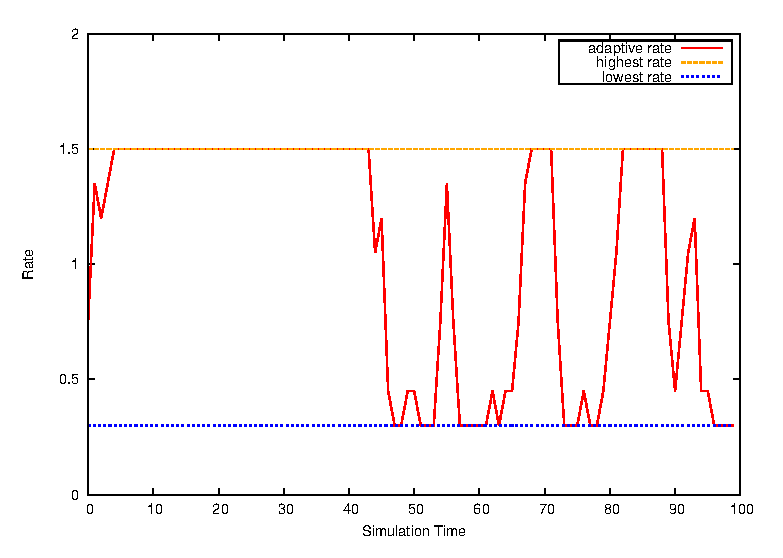
\includegraphics{eps/scenario_2/udp/rate_bw.eps}}
    \caption{Adaptive Rate During Simulation Time}
\end{figure}

\begin{table}[H]
    \centering
    \setlength{\extrarowheight}{2mm}
    \addtolength{\tabcolsep}{3mm}
    \begin{tabular}{c c c}
        \hline \hline
        &  Avg & Stdev \\
        \hline
        AD & 565.797146 & 178.759237 \\
        HI & 749.717684 & 244.254386 \\
        LO & 217.068322 & 25.537143 \\
        \hline
    \end{tabular}
    \caption{Throughput Compare}
\end{table}

Obviously, the three case have a general trend. The rank among three case is same to static model. It also is $HI>AD>LO$. Why their vary trend are same with each other. In this scenario, three case share with the same node movement configuration file. So the trend is no different. The other factor also keep same with static model. So the rank is not change. 

\subsubsection{Loss Rate Compare}
\begin{table}[H]
    \centering
    \setlength{\extrarowheight}{2mm}
    \addtolength{\tabcolsep}{3mm}
    \begin{tabular}{c c c c}
        \hline \hline
        &  Send Packets & Receive Packets & Loss Rate \\
        \hline
        AD & 7505 & 5926 & 0.210393 \\
        HI & 12154 & 6320 & 0.480007 \\
        LO & 3456 & 2731 &  0.209780 \\
        \hline
    \end{tabular}
    \caption{Loss Compare}
\end{table}

The highest loss ratio when the delivery rate is \verb|HI|. It is up to $48\%$. What factor lead to so high loss ratio. What is different by contrast to static scenario? To get the approximate answer, I run \verb|nam|. I found the main difference between these two scenario is that \verb|node_1| may via more than 3 hoc to get communicate with \verb|node_4| in movement scenario. The more hoc, the more probability loss packet. 

\subsubsection{PSNR Compare}
\begin{figure}[H]
    \centering
    \begin{tabular}{l r}
        \resizebox{60mm}{!}{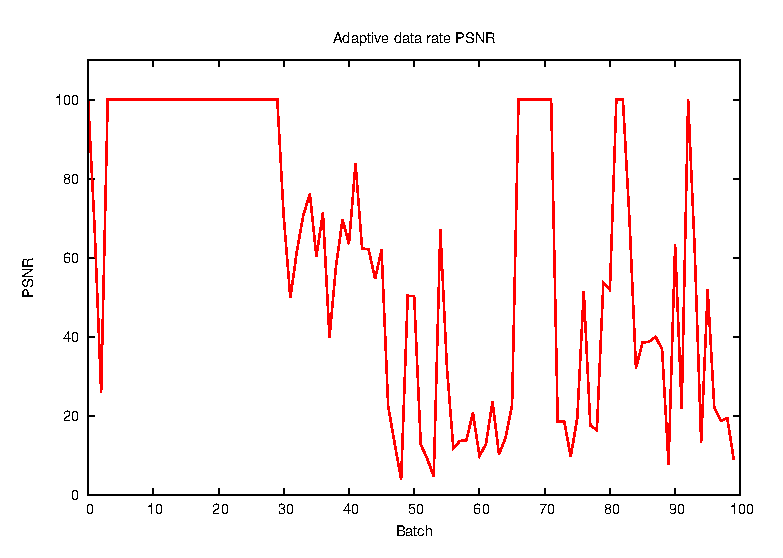
\includegraphics{eps/scenario_2/udp/ad_psnr_bw.eps}} &
        \resizebox{60mm}{!}{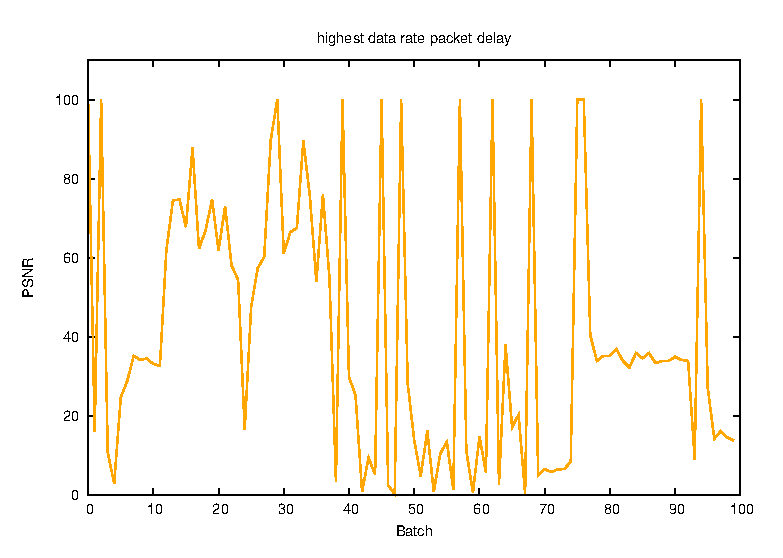
\includegraphics{eps/scenario_2/udp/hi_psnr_bw.eps}} \\
        \multicolumn{2}{c}{\resizebox{60mm}{!}{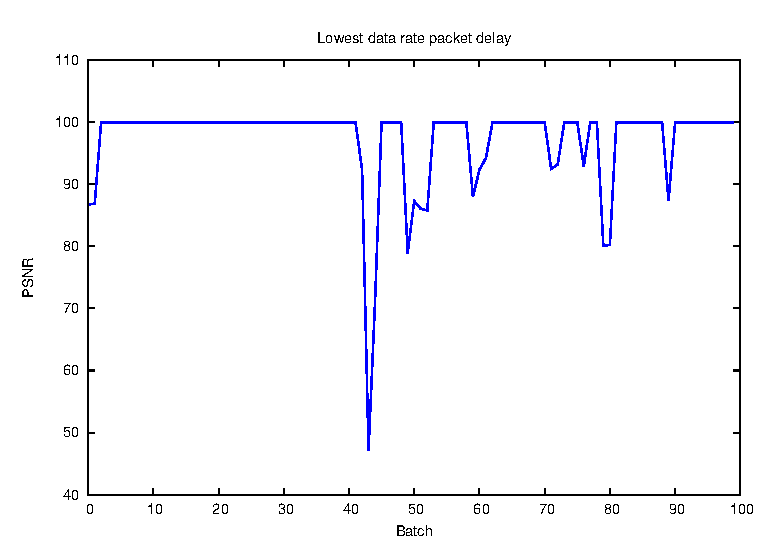
\includegraphics{eps/scenario_2/udp/lo_psnr_bw.eps}}} 
    \end{tabular}
    \caption{PSNR Compare}
\end{figure}

\begin{table}[H]
    \centering
    \setlength{\extrarowheight}{2mm}
    \addtolength{\tabcolsep}{3mm}
    \begin{tabular}{c c c}
        \hline \hline
        &  Avg & Stdev \\
        \hline
        AD & 94.553861 & 20.422601 \\
        HI & 43.137416 & 35.079797 \\
        LO & 97.721715 & 14.298393 \\
        \hline
    \end{tabular}
    \caption{PSNR Compare}
\end{table}

Similar to the above performance almost different with static scenario. \verb|PSNR| also different with static scenario since node is movable. As mention above, \verb|node_1| not always can communicate with \verb|node_4|. Once if the make sense of each other, this stage will keep a short moment. During the stage, the highest transmit maximum data into network. It jitter follow with the relative location of \verb|node_1| and \verb|node_4|.

\newpage
\subsubsection{Summary}
\begin{table}[H]
    \centering
    \setlength{\extrarowheight}{2mm}
    \addtolength{\tabcolsep}{3mm}
     \begin{tabular}{|c|c|c|c|c|}
        \hline 
        \backslashbox{Case}{Performance} & $\overline{Delay}$ & $\overline{Throughput}$ & $\overline{Loss}$ & $\overline{PSNR}$ \\
        \hline
        AD & \textcircled{1}& \textcircled{2} & \textcircled{2} & \textcircled{2}\\
        \hline
        HI & \textcircled{2}& \textcircled{1} & \textcircled{3} & \textcircled{3}\\
        \hline
        LO & \textcircled{3}& \textcircled{3} & \textcircled{1} & \textcircled{1}\\
        \hline
    \end{tabular}
    \caption{Best Performance Sorting}
\end{table}

As like static scenario, I give a rank table to compare these three case. The conclusion is keep same, Comprehensive consideration of various factors, I think the \verb|QOAS_AD| is the best solution among three case.
